% Chapter 2

\chapter{Automatic SynthesiS of Integration Software Tests(ASSIST)} % Main chapter title

\label{Chapter2} % For referencing the chapter elsewhere, use \ref{Chapter2} 

\lhead{Chapter 2. \emph{ASSIST}} % This is for the header on each page - perhaps a shortened title

%----------------------------------------------------------------------------------------

\section{Overview}
Automatic SynthesiS of Integration Software Tests(ASSIST) aims to provide a new solution using unit tests and acceptance tests. It fulfills various objectives in order to achieve the aim.

\subsection{Synthesis of Fewer and Tighter Integration Tests}
There is a need to decrease the number of integration tests on synthesis of which they are more effective which also means it has a increased power of finding bugs. This is because as we discussed randomly generating integration tests for all combinations of components increases costs in terms of time and resources. Thus, one of the objective is to produce an acceptable number of integration tests with a high bug finding power.

To reach this goal, the system will use the acceptance and unit tests to get models that can enhance the synthesis of integration tests. The Application Under Test(AUT) is run and execution traces are collected using a runtime monitoring system. It will generate models that describe the relationship between properties of input data for AUT and frequent interactions between various components, obtained by mining patterns of method invocations in execution traces. \emph{The system reduces this computationally intensive task by pruning the sequences of components that are not tightly integrated assuming that loosely integrated components have lesser possibility of integration bugs}. The above objective is the goal of the project and is explained in detail in Chapter\ref{Chapter4}.
 
ASSIST will prioritize synthesis of those integration tests which have interactions among components in the AUT like if they exchange more data or if they invoke each other's methods during execution of system with various input data, or execution path in object of one class affect the object of another class. Thus these types of components are considered tighter and are intuitively lead us to integration bugs.
 
\subsection{Meaningful Oracles}
Integration tests are more meaninful if they have better \emph{oracles} (methods for checking of the AUT have given correct outputs on a particular execution  \cite{Baresi:Oracles}). Generating oracles is one of the most difficult issue of general software testing \cite{Baresi:Oracles,Peters1994,Richardson-icse92,Richardson1994,dillon-sigsoft94}. \cite{MYSOA:07} suggests that as much as 25\% of the time is spent in testing oracles by many companies.

We can create an oracle by capturing the state at the very end of the completion of execution of the last method in an AUT but it would be a very huge oracle in terms of size and even the states will be very large to manage and maintain for each integration test. It is kind of misguiding if the unused values do not match, testers may keep finding errors which even donot occur. Thus, it is diffcult to maintain and evolve tests without specific fields and values in an oracle \cite{Daniel:2009:RSR:1747491.1747538}.

System overcomes the issue by projecting carved AUT states onto field used in assertions(\emph{assert} statements) of the unit tests for synthesized integration tests. These are the fields that hold data flow and control flow informtion. By using symbolic execution \cite{Boyer:1975:SFS:800027.808445,DBLP:journals/cacm/King76,DBLP:journals/tse/Clarke76,csallner08dysy,godefroid05dart,sen06cute,SYMEX:81,KING:71}
we can deal with this objective.

\subsection{Evaluate}
To evaluate the effectiveness of the results Mutation Integration will be used.

%----------------------------------------------------------------------------------------

\section{Organization}
\label{Organization}
Below shown and mentioned are the various steps in the ASSIST project.

\begin{figure}[h]
\centering
 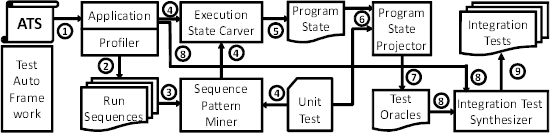
\includegraphics{Workflow}
\caption{The architecture and workflow of ASSIST.}
\label{workflow}
\end{figure}

 
\begin{enumerate}
\item The Application Test Suite(ATS) comprises of AUT, unit and acceptance tests and input data for these tests.
\item AUT is run using with a profiler which collects \textit{run sequences} (execution traces) which contain method names and class names.
\item Run Sequences are analysed by Sequence Pattern Miner that mines patterns from the various runs.\label{3}
\item A subset of the most informative run sequences are submitted to the State Carver.\label{4}
\item State Carver extracts the state of heap memory in the execution of the AUT before the extracted patterns are run.
\item Using unit tests and state of the system Program State Projector determines test oracles.
\item These oracles and source code of AUT are used by Integration Test Synthesizer. 
\item Integration tests are outputted.
\end{enumerate}